\chapter{阀盖立体图}

{\bfseries 学习目标}
\begin{itemize}
\item 学习利用xline命令的角度选项绘制图形
\item 学习利用arc命令绘图形
\item 学习利用union命令构建三维模型
\item 掌握基本几何体的三视图表达
\end{itemize}

{\bfseries 任务要求}
\begin{itemize}
\item 根据图\ref{fig:tiaoyafafagai}所示的杯零件图,用拉伸法建立调压阀杯零件的三维模型
\end{itemize}

\noindent
\begin{figure}[htbp]
\centering
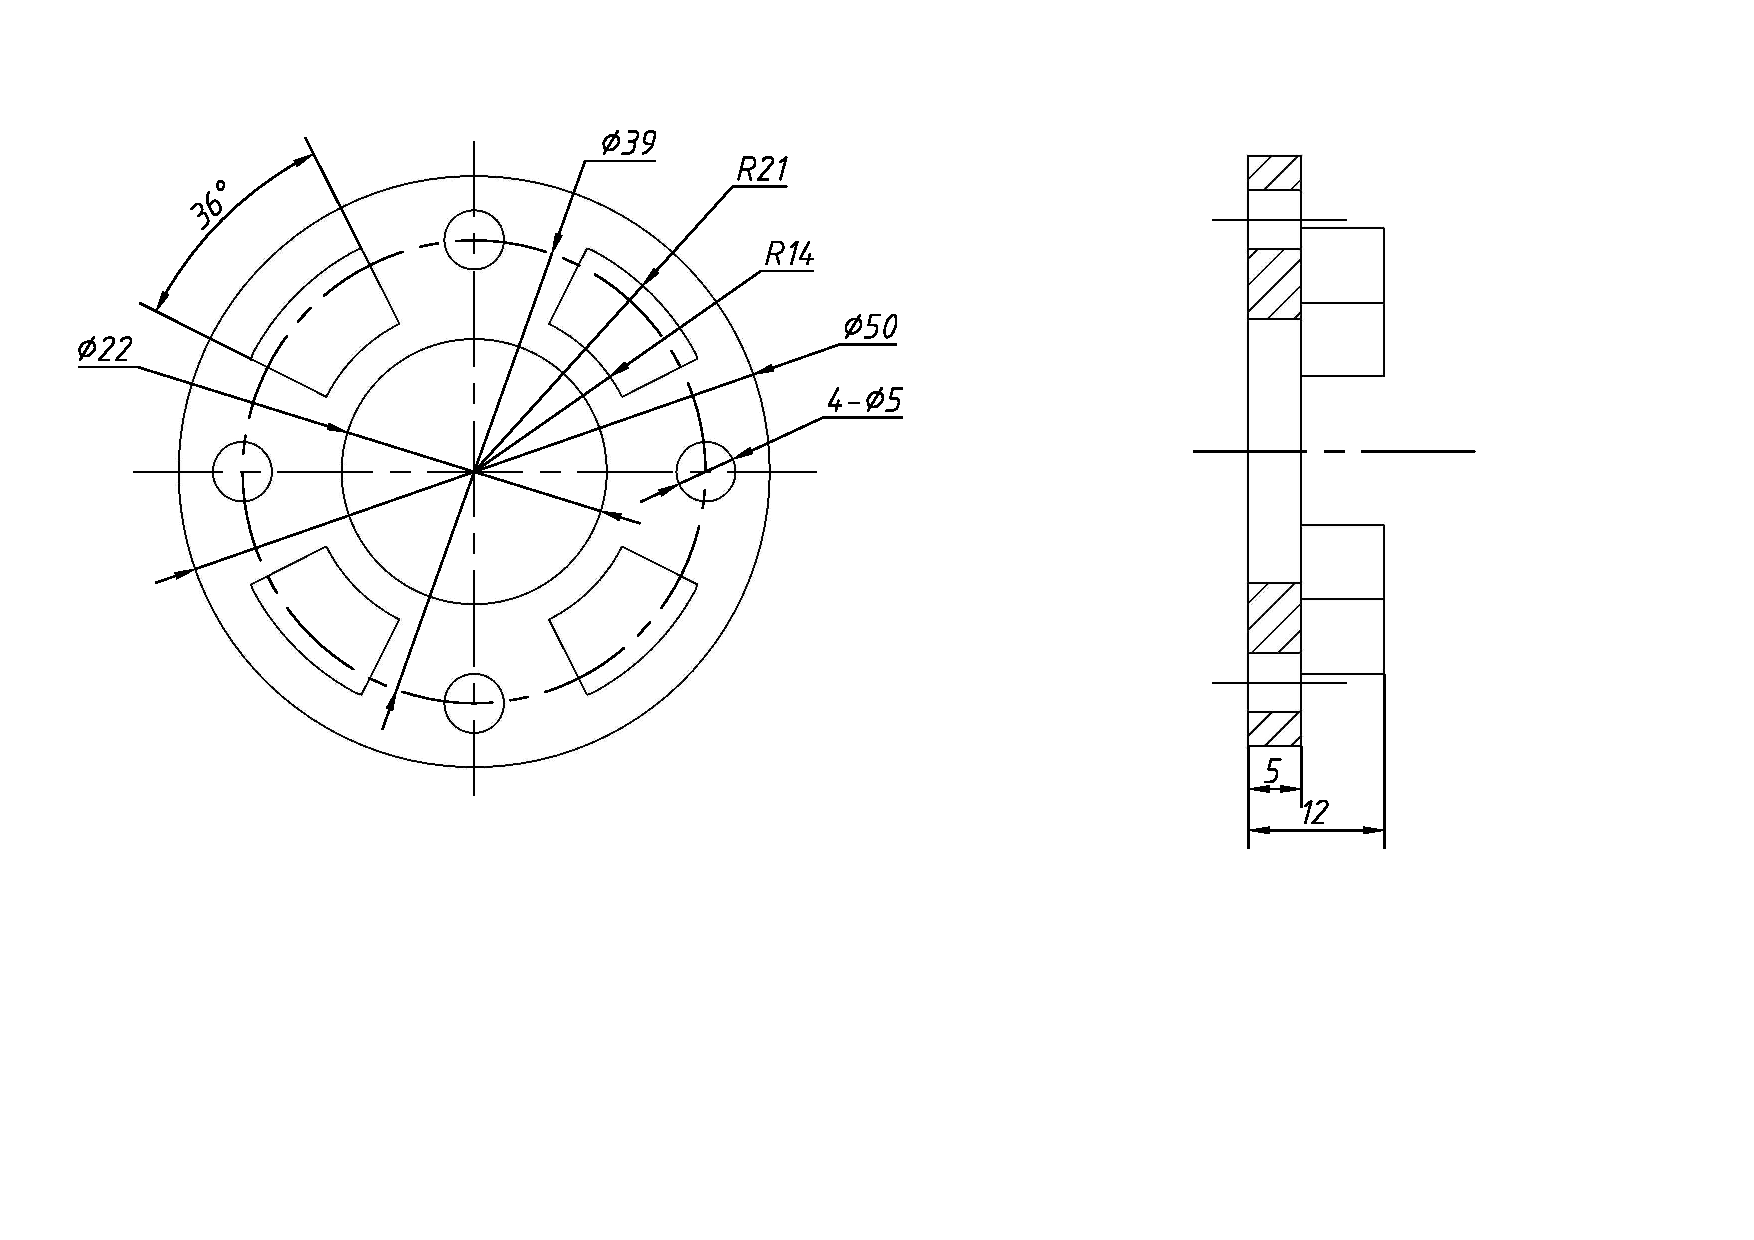
\includegraphics[scale=0.6]{tiaoyafafagai.pdf}
\caption{杯零件图}\label{fig:tiaoyafafagai}
\end{figure}
\endinput